\documentclass[10pt,a4paper]{article}
\usepackage{ctex}
%\usepackage{newtxtext,newtxmath} % Times New Roman font for academic papers
\usepackage{fancyhdr}
\usepackage{booktabs}
\usepackage{graphicx}
\usepackage{amsmath}
\usepackage{float}
\usepackage{xcolor}
\usepackage{listings}
\usepackage{multirow}
\usepackage{diagbox}
\usepackage[table]{xcolor}
\usepackage{subcaption}
\usepackage{tikz}
\usetikzlibrary{shapes,arrows,positioning}
\usepackage[colorlinks,linkcolor=blue]{hyperref} % For inserting hyperlinks

% Set figure and table captions to English
\renewcommand{\figurename}{Figure}
\renewcommand{\tablename}{Table}

% Document page margin settings
\usepackage[a4paper]{geometry}
\geometry{top=1in}
\geometry{bottom=1in}
\geometry{left=0.75in}
\geometry{right=0.75in}   % Set top, bottom, left, and right margins
\geometry{marginparwidth=1.75cm}    % Set margin note distance (comments, markers, etc.)

% Set page header
\pagestyle{fancy}
\fancyhf{}
\lhead{\footnotesize Final Report}
\chead{\footnotesize Personalized News Headline Generation}
\rhead{\thepage}
\renewcommand{\headrulewidth}{0.4pt}

% Code settings
\lstset{
    basicstyle=\ttfamily\small,
    numbers=left,
    numberstyle=\tiny,
    keywordstyle=\color{blue},
    commentstyle=\color{green!60!black},
    stringstyle=\color{red},
    breaklines=true,
    frame=single,
    showstringspaces=false
}

\begin{document}

\begin{center}
    \LARGE{\textbf{Personalized News Headline Generation:\\ PENS Baseline Method Improvement and Implementation of Prompt Engineering Approach}}
    
    \vspace{0.5cm}
    \large{Luofan Wang, Shouhe Zhu}
    
    \large{June 23, 2025}
\end{center}

\section{Overview of Completion Status}
Our group selected the "Personalized Headline Generation Task" topic and conducted collaborative development through a GitHub repository. We have completed two alternative technical approaches, including PENS baseline method reproduction and improvement, and a prompt engineering-based large language model personalized generation method. We now have completed runnable code with clear README documentation and an innovative evaluation scheme designed by ourselves.

\section{PENS Baseline Method Reproduction and Improvement}
\subsection{Environment Setup}
The local environment has been configured with CUDA 11.8 to meet the GPU acceleration requirements for deep learning tasks. Considering that the project involves multiple deep learning libraries (including PyTorch, Transformers, NumPy, etc.), to ensure stability and reproducibility of dependency management, we adopted Conda as the environment management tool and built an independent virtual environment based on the requirements.txt file provided by the baseline project.

\subsection{Baseline Method Analysis}
\subsubsection{Overall Architecture}
The project follows a classic three-stage pipeline architecture: Data Preprocessing (Preprocess) $\rightarrow$ User Modeling (UserEncoder) $\rightarrow$ Personalized Generation (Generator). Initially, raw data is stored in the 'data/' directory. First, the 'Preprocess' component cleans, transforms, and structures the raw data, outputting to the 'data2/' directory, which serves as the direct data source for all subsequent model training. Then the 'UserEncoder' and 'Generator' components respectively perform model training and save the trained models (i.e., component outputs) in corresponding subdirectories under the 'runs/' directory. In this process, downstream components explicitly depend on upstream component outputs: 'UserEncoder' depends on 'data2/' data, while 'Generator' depends on both 'data2/' data and the model trained by 'UserEncoder'.

\subsubsection{Core Component Analysis}
\textbf{Data Preprocessing (Preprocess):} In the PENS personalized news headline generation project, the data preprocessing (Preprocess) component is the starting point of the entire workflow, with core logic concentrated in pensmodule/Preprocess/preprocess.ipynb. The main responsibility of this component is to convert raw, unstructured news text and user behavior logs into standardized numerical formats acceptable to deep learning models. Internally, it consists of multiple functional modules that, while not independent Python scripts, form a complete pipeline through sequential execution of Jupyter Notebook code cells. First, the environment configuration module imports necessary libraries (such as pandas, numpy, nltk, torch) and defines global hyperparameters (such as MAX\_CONTENT\_LEN, WORD\_FREQ\_THRESHOLD, etc.), establishing unified standards for the data processing pipeline. Next, the news parsing module (read\_news) reads the raw news.tsv file, performs text cleaning, tokenization, word frequency statistics, and constructs core dictionary mappings like word\_dict, category\_dict, and news\_index. Subsequently, these dictionaries and index information are serialized and saved to the /data2 directory (as shown in Figure \ref{fig:processed_data}), serving as the first data checkpoint in the project. To meet downstream model input format requirements, Preprocess generates different data representations for the user encoder (UserEncoder) and headline generator (Generator). The former generates fixed-length news headline, content, and category ID sequences saved as .npy files, while the latter constructs source-target pairs required by Seq2Seq models, including content input, headline input and output sequences. Additionally, the component builds word embedding matrices for the project by loading pre-trained GloVe vectors, and processes user click logs to generate user click history and training samples, including positive and negative sample pairs. Finally, these user data are also serialized and stored, becoming the foundation for subsequent model training. The entire Preprocess component ensures data processing continuity, structural clarity, and downstream reusability through a combination of memory variable passing and file system persistence, serving as a solid data foundation for achieving the project's personalized generation capabilities.

\begin{figure}[H]
  \centering
  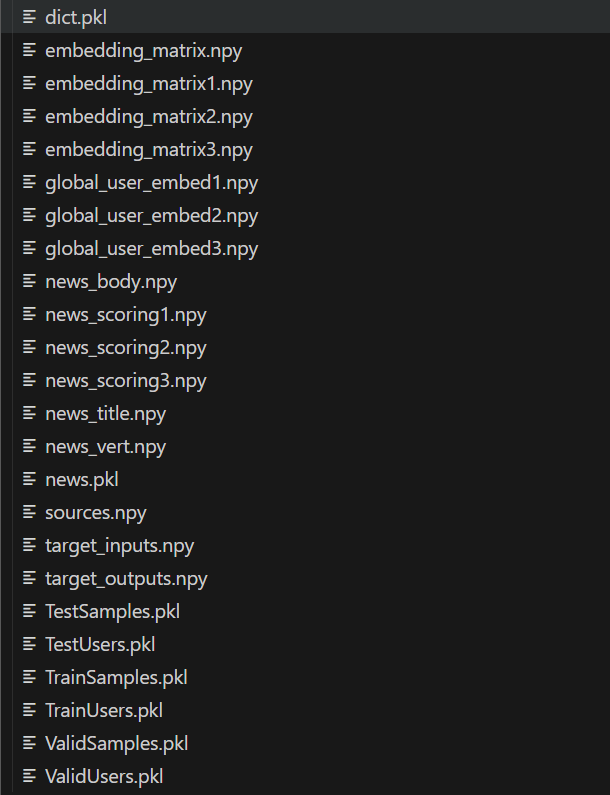
\includegraphics[width=10.5cm]{fig/processed_data.png}
  \caption{Preprocessed Data}\label{fig:processed_data}
\end{figure}

\textbf{User Encoder (UserEncoder):}
This component undertakes the core responsibility of "understanding users" with the goal of converting users' historical click behaviors into a fixed-dimensional user interest vector (User Vector) to guide downstream headline generation models. This component takes structured data generated by the Preprocess component as input and ultimately outputs a trained deep learning model. The logic is distributed across multiple Python files and coordinated by a Jupyter Notebook (pipeline\_Train\_Test.ipynb). The workflow first involves data.py handling data loading, constructing .npy and .pkl files into PyTorch-compatible Dataset and DataLoader, where each training sample includes candidate news, user click history, and their labels. Subsequently, modules.py defines general network structures such as MultiHeadAttention and AttentionPooling, providing building blocks for core models (like NRMS) in model.py. model.py defines specific structures for news encoders and user encoders, utilizing word embedding initialization and attention mechanisms to extract user interest representations. The auxiliary module utils.py provides accuracy evaluation functions during model training, while the overall training process is concentrated in pipeline\_Train\_Test.ipynb, including environment configuration, data loading, model initialization, iterative training, performance evaluation, and model saving. The entire UserEncoder component is highly modular with clear logic, and its training outputs are saved in the runs/userencoder/ directory (as shown in Figure \ref{fig:user_encode}), serving as important input for the downstream Generator component's personalized headline generation. This design, characterized by clear division of labor and low coupling, facilitates easy maintenance, debugging, and replacement of components.

\begin{figure}[H]
  \centering
  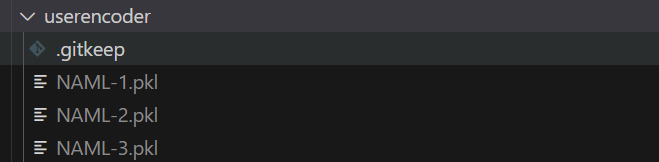
\includegraphics[width=10cm]{fig/user_encode.png}
  \caption{Encoder Output}\label{fig:user_encode}
\end{figure}

\textbf{Personalized Generator (Generator):}
This component is the final execution unit of the entire system, with the main task of integrating structured data from Preprocess and user interest vectors provided by UserEncoder to generate personalized news headlines that both conform to news content and match user preferences. This component adopts the classic "pre-training-fine-tuning" two-stage strategy common in modern natural language generation tasks, consisting of multiple functional modules and unified scheduling through pipeline\_pretrain\_train\_test.ipynb. First, the configuration file config.json provides global definitions of model structure and training hyperparameters; the data loading module data.py converts structured data into PyTorch Dataset suitable for training, where Seq2SeqDataset is used for general pre-training, and ImpressionDataset loads user click history and news vectors for personalized fine-tuning. The model's underlying components are distributed in encoder.py, decoder\_pointer.py, and modules.py, respectively defining encoders, decoders with pointer mechanisms, and general attention layers, implementing effective representation of input news text and personalized control capabilities. The HeadlineGen class in model.py integrates the above modules into a complete trainable model, whose forward function implements the entire process of encoding news text and combining user interest vectors to decode and generate headlines. Training logic is supported by modules like train.py and eval.py, encapsulating optimizers, loss functions, fine-tuning logic, performance evaluation, and Beam Search generation strategies. The entire training and evaluation process unfolds orderly in the Jupyter Notebook: first using Seq2SeqDataset for pre-training to learn general headline generation capabilities; then loading the trained UserEncoder model for fine-tuning, injecting user interest vectors into the generation process to achieve true personalized generation, and saving the final model in the runs/ directory (as shown in Figure \ref{fig:model_weight}).

\begin{figure}[H]
  \centering
  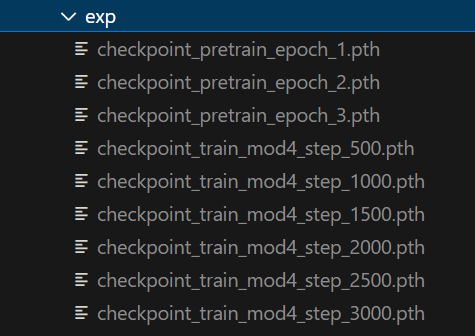
\includegraphics[width=6.5cm]{fig/model_weight.png}
  \caption{Trained Model Weights}\label{fig:model_weight}
\end{figure}

\subsection{Baseline Method Improvements}
\textbf{Solving Compatibility Issues in Original Code:}
When adapting project code to PyTorch 2.0 and above versions, we found compatibility issues with the original model loading approach. Specifically, the original code directly used torch.load(checkpoint\_path) for model restoration when loading trained model checkpoints. However, starting from PyTorch 2.0, torch.load() added a new default parameter weights\_only=True, meaning it only loads model weights by default without restoring the model object structure itself. Since the original code did not explicitly specify weights\_only=False, this would cause checkpoint['model'] to return None or an empty dictionary during model loading, triggering errors when subsequently attempting to call model attributes, perform inference, or fine-tuning operations. Therefore, to ensure stable code execution and complete model restoration, we need to explicitly pass the weights\_only=False parameter when loading checkpoints (as shown in Figure \ref{fig:model_loader}), ensuring both model structure and weights are loaded together. This fix is crucial for the normal operation of subsequent modules (such as fine-tuning and inference in the personalized generator).

\begin{figure}[H]
  \centering
  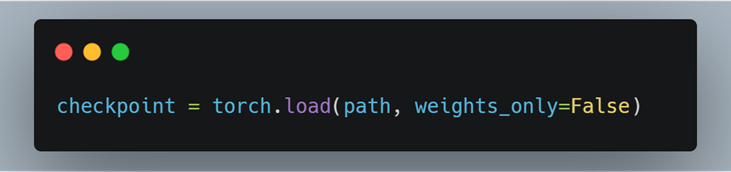
\includegraphics[width=10cm]{fig/load_new.png}
  \caption{Improved Model Loading Method}\label{fig:model_loader}
\end{figure}

\textbf{Training Method Optimization:}
During reproduction and execution of the original project training process (including UserEncoder training and Generator pre-training/fine-tuning), we observed severely suboptimal local GPU utilization. During training, GPU occupancy was below 10\% most of the time, and power consumption was also near idle state, with only brief increases at certain intervals, but peak values were also low. This "GPU idle" phenomenon indicates that the training bottleneck is not in model computation but in the data transmission process. Analysis of the data loading process revealed that the original DataLoader used a single-threaded loading strategy without any memory acceleration mechanisms, causing CPU data preparation speed to be unable to match GPU computation speed, frequently blocking GPU waiting for input. To address this, we made two optimizations to the training data loading process (as shown in Figure \ref{fig:data_loader}): first, setting the DataLoader's num\_workers parameter to a larger value supported by the system (such as 20), enabling multi-threaded data loading to improve data reading and preprocessing speed; second, enabling pin\_memory=True to load data into pinned memory, accelerating CPU to GPU data transfer speed. This series of improvements significantly enhanced system throughput, maintaining GPU occupancy at 97\%$\sim$100\% for extended periods, improving overall training efficiency by approximately double, especially showing significant improvements in iteration speed during data preprocessing, model pre-training, and personalized fine-tuning stages.

\begin{figure}[H]
  \centering
  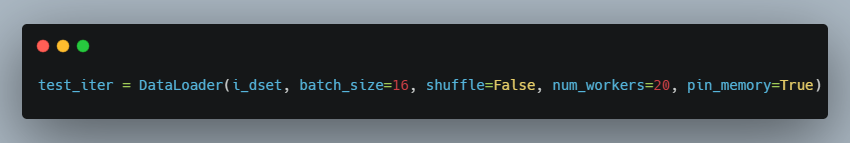
\includegraphics[width=15cm]{fig/dataloader.png}
  \caption{Improved Data Loading Method}\label{fig:data_loader}
\end{figure}

\textbf{New Functional Modules:}
To enhance project usability and interactivity, we added a new functional module named predict\_with\_trained\_model.ipynb for model inference applications and result output. This module allows users to directly load trained personalized headline generation models after training completion and perform headline generation tasks on specified input data (which can be original news content or user-defined text). Generation results are automatically saved in the generated\_titles.txt file in the current directory for easy review and subsequent analysis. Additionally, if users provide corresponding "reference headlines" (i.e., manually written or existing real headlines), the system will automatically call built-in evaluation functions to perform ROUGE metric scoring on generation results, quantifying model generation quality. The addition of this module not only enhances project practicality but also provides convenience for actual deployment, user interaction, and performance evaluation.

\subsection{Experimental Results}
After completing full reproduction of the baseline method, we conducted systematic evaluation of model performance at different training stages, with relevant experimental results saved in the /docs0 directory. Main evaluation metrics include reward values obtained by the model during training (as shown in Figure \ref{fig:reward}) and ROUGE metric score changes on the validation set (as shown in Figure \ref{fig:rouge}). Figure \ref{fig:reward} shows the reward curve during training, where we can observe that the model's reward increases rapidly in early training stages and then gradually stabilizes; Figure \ref{fig:rouge} reflects the similarity trend between model generation results and reference headlines at different training steps.

From experimental results, if using ROUGE scores as the sole performance evaluation standard, we can clearly observe that the model reaches optimal performance around training step 2000, where ROUGE-1, ROUGE-2, and ROUGE-L scores all reach peak values under the current training process, indicating that headlines generated by the model at this stage are closest to manually created reference headlines in terms of content coverage, information completeness, and language structure.

\begin{figure}[H]
  \centering
  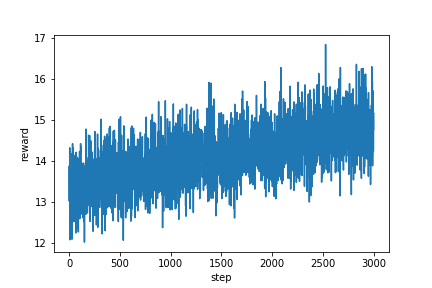
\includegraphics[width=7cm]{fig/reward.png}
  \caption{Training Reward vs. Training Steps}\label{fig:reward}
\end{figure}

\begin{figure}[H]
  \centering
  \begin{subfigure}{0.32\textwidth}
    \centering
    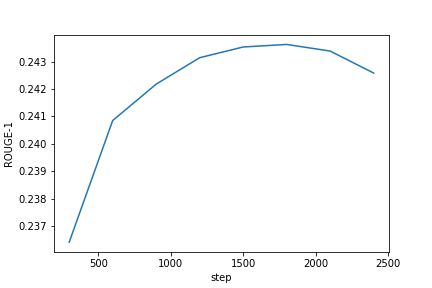
\includegraphics[width=\textwidth]{fig/rouge1.png}
  \end{subfigure}
  \hfill
  \begin{subfigure}{0.32\textwidth}
    \centering
    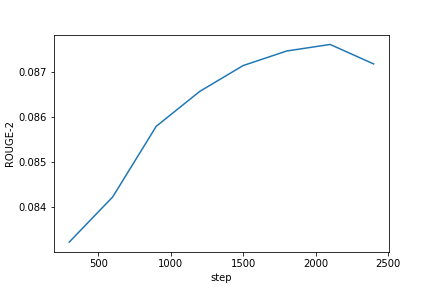
\includegraphics[width=\textwidth]{fig/rouge2.png}
  \end{subfigure}
  \hfill
  \begin{subfigure}{0.32\textwidth}
    \centering
    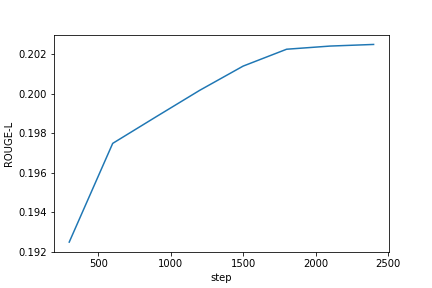
\includegraphics[width=\textwidth]{fig/rougel.png}
  \end{subfigure}
  \caption{ROUGE Scores vs. Training Steps}\label{fig:rouge}
\end{figure}

Furthermore, to verify the model's generation capabilities in real application scenarios, this project called the trained personalized headline generation model to conduct experiments on a set of custom news sample data, generating news headlines with user preferences. During experiments, input data included custom news content, while associated user click history information reused original data. The model comprehensively judged user interests based on this information and generated headline text that better matched user reading preferences while ensuring semantic reasonableness.

Figure \ref{fig:ref} shows manually created reference headlines for this set of custom news samples; Figure \ref{fig:gen} shows personalized headline results generated by the model under the above input conditions. Through comparison, we find that generated headline 1 covers key news information while also showing certain user preference tendencies in expression and word choice, such as more attractive wording and word order that better matches user click tendencies. However, headlines 2 and 3 performed poorly, not only failing to use more attractive wording but even losing key information from original news headlines. This shows that the model's generalizability and practicality still need strengthening.

\begin{figure}[H]
  \centering
  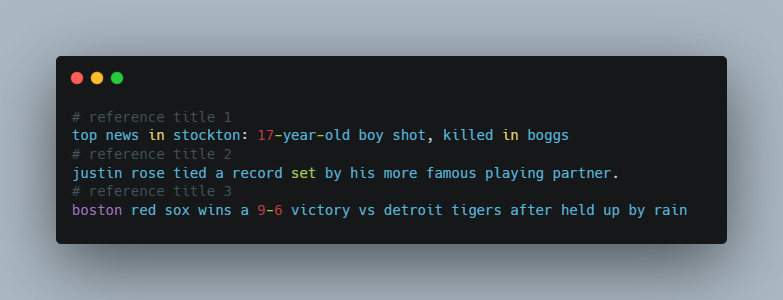
\includegraphics[width=15cm]{fig/reference.png}
  \caption{Reference Headlines}\label{fig:ref}
\end{figure}
\begin{figure}[H]
  \centering
  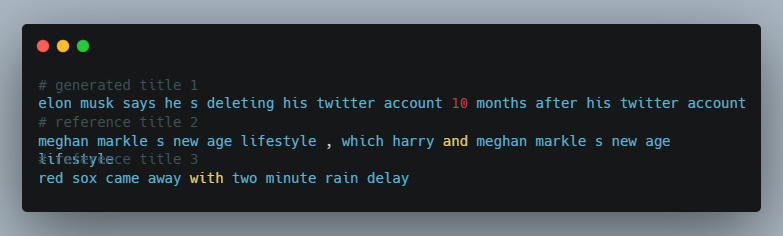
\includegraphics[width=15cm]{fig/generated.png}
  \caption{Generated Headlines}\label{fig:gen}
\end{figure}

\section{Prompt-engineering-based Method}
\subsection{Relay API Platform Construction}
To achieve unified management and efficient calling of large language model APIs, this project built the ChavAPI relay platform (\url{https://api.chavapa.com}) through self-built servers based on existing open-source projects One-API and DeepClaude on Github. The construction of this platform provided solid technical support for the prompt engineering method.

The ChavAPI platform adopts a distributed architecture design and achieves high availability through Docker containerized deployment. Core platform functions include: multi-model unified interface encapsulation, intelligent load balancing, request throttling and quota management, real-time monitoring and logging, etc. In API key management, the platform supports multi-channel key polling usage, effectively distributing request pressure, and ensures key security through encrypted storage. For load balancing strategies, the system dynamically adjusts request allocation based on metrics such as response time and success rate of various API providers, ensuring service stability. Meanwhile, the platform provides detailed usage statistics and cost analysis functions, supporting precise billing by project and by user, providing strong support for project budget control.

Additionally, the ChavAPI platform strictly follows OpenAI API standards in compatibility design, enabling project code to seamlessly connect with different large language model service providers, including mainstream models like DeepSeek, Gemini series, Claude series, etc. This unified interface design not only simplifies code development processes but also provides convenience for potential horizontal model comparison experiments.

\begin{figure}[H]
\centering
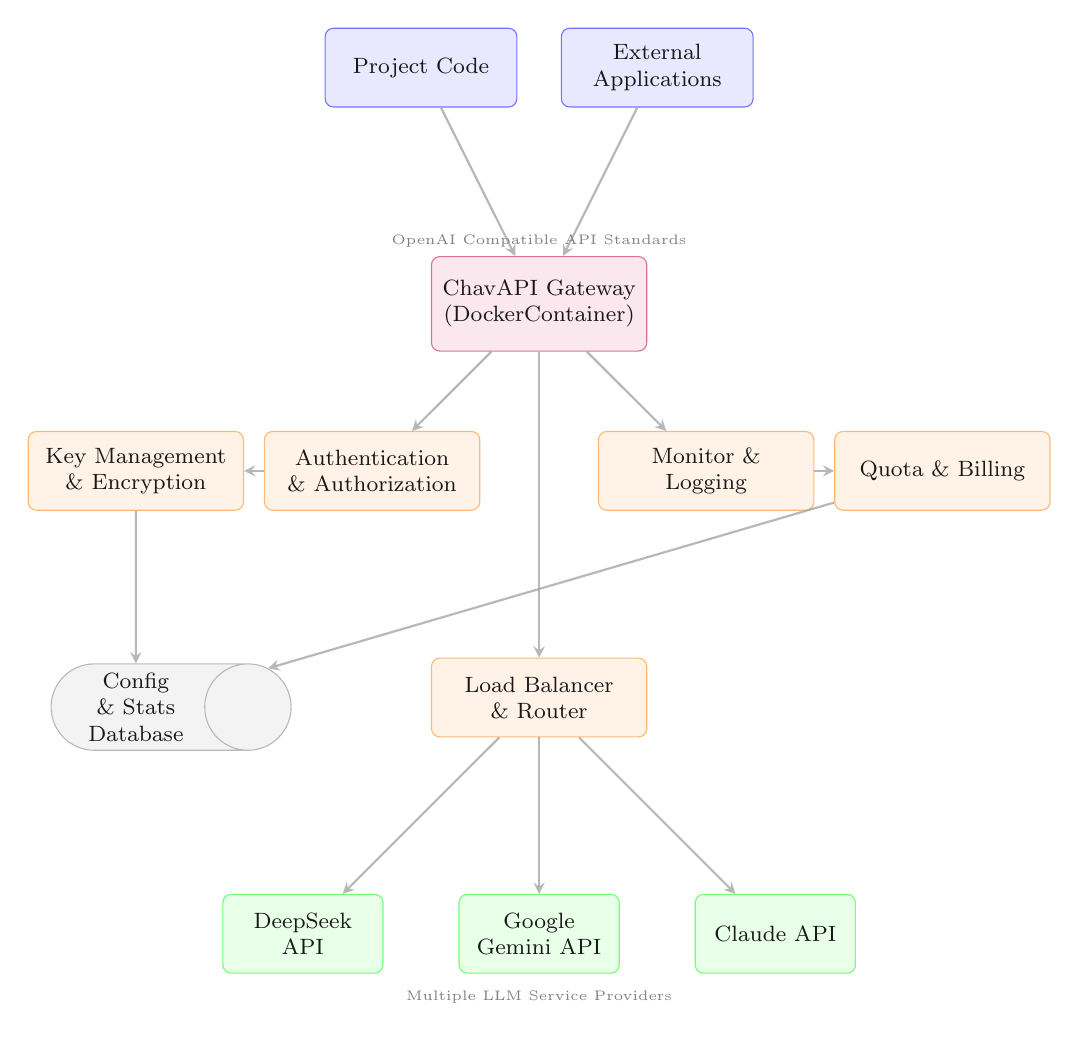
\begin{tikzpicture}[
    node distance=3cm,
    auto,
    client/.style={rectangle, draw=blue!60, fill=blue!10, text width=2.2cm, text centered, rounded corners=3pt, minimum height=1cm, font=\footnotesize, opacity=0.9},
    gateway/.style={rectangle, draw=purple!60, fill=purple!10, text width=2.5cm, text centered, rounded corners=3pt, minimum height=1.2cm, font=\footnotesize, opacity=0.9},
    service/.style={rectangle, draw=orange!60, fill=orange!10, text width=2.5cm, text centered, rounded corners=3pt, minimum height=1cm, font=\footnotesize, opacity=0.9},
    provider/.style={rectangle, draw=green!60, fill=green!10, text width=1.8cm, text centered, rounded corners=3pt, minimum height=1cm, font=\footnotesize, opacity=0.9},
    db/.style={cylinder, draw=gray!60, fill=gray!10, text width=1.5cm, text centered, minimum height=1cm, font=\footnotesize, opacity=0.9},
    arrow/.style={->,>=stealth, draw=gray!70, opacity=0.8, thick}
]

% Client Layer
\node [client] (client1) {Project Code};
\node [client, right of=client1] (client2) {External Applications};

% Gateway Layer
\node [gateway, below of=client1, xshift=1.5cm] (gateway) {ChavAPI Gateway\\(DockerContainer)};

% Service Layer
\node [service, below left of=gateway] (auth) {Authentication \& Authorization};
\node [service, below of=gateway, node distance=5cm] (balance) {Load Balancer \& Router};
\node [service, below right of=gateway] (monitor) {Monitor \& Logging};

% Management Layer
\node [service, left of=auth] (key) {Key Management \& Encryption};
\node [service, right of=monitor] (quota) {Quota \& Billing};

% Database
\node [db, below of=key] (database) {Config \& Stats Database};

% Provider Layer
\node [provider, below of=balance, xshift=-3cm] (deepseek) {DeepSeek API};
\node [provider, below of=balance] (google) {Google Gemini API};
\node [provider, below of=balance, xshift=3cm] (claude) {Claude API};

% Arrows - Client to Gateway
\draw [arrow] (client1) -- (gateway);
\draw [arrow] (client2) -- (gateway);

% Arrows - Gateway to Services
\draw [arrow] (gateway) -- (auth);
\draw [arrow] (gateway) -- (balance);
\draw [arrow] (gateway) -- (monitor);

% Arrows - Service connections
\draw [arrow] (auth) -- (key);
\draw [arrow] (monitor) -- (quota);
\draw [arrow] (key) -- (database);
\draw [arrow] (quota) -- (database);

% Arrows - Load Balancer to Providers
\draw [arrow] (balance) -- (deepseek);
\draw [arrow] (balance) -- (google);
\draw [arrow] (balance) -- (claude);

% Labels for API standards
\node [above of=gateway, node distance=0.8cm, font=\tiny, text=gray] {OpenAI Compatible API Standards};
\node [below of=google, node distance=0.8cm, font=\tiny, text=gray] {Multiple LLM Service Providers};

\end{tikzpicture}
\caption{ChavAPI Platform Architecture}
\label{fig:chavapi_architecture}
\end{figure}

\subsection{Local Environment Setup}
The environment configuration for the prompt engineering method is relatively simple, mainly relying on the Python ecosystem and cloud API services. Local environment setup includes Python 3.8+ runtime, core dependency package installation (OpenAI, Pandas, NumPy, Rouge-Score, Matplotlib, etc.), and Jupyter Notebook development environment configuration. Compared to the baseline method, this solution does not require complex deep learning environment configuration, avoiding technical difficulties such as CUDA version compatibility and GPU memory management.

API configuration management adopts a template design, providing standard configuration templates through \texttt{api\_config\_template.py}. Users only need to copy to \texttt{api\_config.py} and fill in corresponding API keys to complete configuration. Configuration files support multi-model parameter definitions, including differentiated settings for reasoning models (such as DeepSeek-R1 series) and chat models (such as DeepSeek-Chat series). The system automatically adjusts key configurations such as maximum token count and temperature parameters based on model types, ensuring optimal performance for different models.

The project adopts a modular directory structure design with core components including data processor (\texttt{data\_processor.py}), prompt generator (\texttt{prompt\_generator.py}), LLM client (\texttt{llm\_client.py}), evaluator (\texttt{evaluator.py}), etc. Each module has clear responsibilities and is easy to maintain and extend. Output directories are organized by function categories, including subdirectories for preprocessed data, generated headlines, evaluation results, etc., ensuring orderly management of experimental data.

\subsection{Prompt Engineering Method Analysis}
\subsubsection{Overall Architecture}
The prompt engineering method adopts a "data-driven + intelligent prompting" technical approach, with the overall architecture divided into four core stages: data preprocessing and user profiling construction, adaptive prompt generation, large language model API calling and content generation, multi-dimensional intelligent evaluation. Unlike traditional deep learning methods, this architecture fully utilizes the language understanding and generation capabilities of large language models, implementing personalized content generation through carefully designed prompt templates, avoiding complex model training processes.

\begin{figure}[H]
\centering
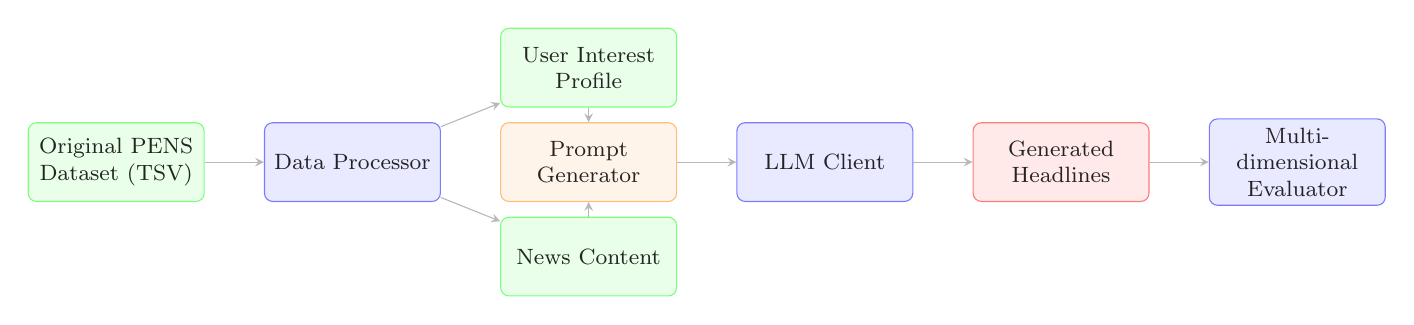
\begin{tikzpicture}[
    node distance=3cm,
    auto,
    block/.style={rectangle, draw=blue!60, fill=blue!10, text width=2cm, text centered, rounded corners=3pt, minimum height=1cm, font=\footnotesize, opacity=0.85},
    data/.style={rectangle, draw=green!60, fill=green!10, text width=2cm, text centered, rounded corners=3pt, minimum height=1cm, font=\footnotesize, opacity=0.85},
    process/.style={rectangle, draw=orange!60, fill=orange!10, text width=2cm, text centered, rounded corners=3pt, minimum height=1cm, font=\footnotesize, opacity=0.85},
    result/.style={rectangle, draw=red!60, fill=red!10, text width=2cm, text centered, rounded corners=3pt, minimum height=1cm, font=\footnotesize, opacity=0.85},
    arrow/.style={->,>=stealth, draw=gray!70, opacity=0.8}
]

% Nodes
\node [data] (dataset) {Original PENS Dataset (TSV)};
\node [block, right of=dataset] (processor) {Data Processor};
\node [process, right of=processor] (prompt) {Prompt Generator};
\node [block, right of=prompt] (llm) {LLM Client};
\node [result, right of=llm] (output) {Generated Headlines};
\node [block, right of=output] (eval) {Multi-dimensional Evaluator};

% Additional nodes for data flow
\node [data, above of=prompt, node distance=1.2cm] (profile) {User Interest Profile};
\node [data, below of=prompt, node distance=1.2cm] (content) {News Content};

% Arrows
\draw [arrow] (dataset) -- (processor);
\draw [arrow] (processor) -- (profile);
\draw [arrow] (processor) -- (content);
\draw [arrow] (profile) -- (prompt);
\draw [arrow] (content) -- (prompt);
\draw [arrow] (prompt) -- (llm);
\draw [arrow] (llm) -- (output);
\draw [arrow] (output) -- (eval);

\end{tikzpicture}
\caption{Prompt Engineering Method Workflow}
\label{fig:prompt_workflow}
\end{figure}

The system workflow is as follows: First, the data processor extracts user historical click sequences from the original PENS dataset and constructs user interest profiles through statistical analysis, including main interest categories, preference weights, and other information; Subsequently, the prompt generator dynamically constructs personalized prompt templates based on target news content and user profiles; Next, the LLM client calls large language model APIs to generate personalized headlines based on the generated prompts; Finally, the evaluator uses multiple methods including ROUGE automatic evaluation and LLM intelligent evaluation to comprehensively evaluate generation results.

\subsubsection{Core Component Analysis}
\textbf{Data Preprocessing Module (DataProcessor):} This module is responsible for extracting user behavior sequences and news content from original TSV format data, constructing structured data suitable for prompt engineering. Core functions include user historical click sequence extraction, interest category statistical analysis, test sample preparation, etc. Unlike complex feature engineering in baseline methods, this module focuses on preserving and organizing semantic information, converting original text data into easily understandable natural language descriptions. The user interest extraction algorithm analyzes news category distributions in click history, calculates click frequency and weights for each category, and determines users' main interest areas. During data processing, the system truncates news content length (limited to within 400 characters) to ensure prompt total length is controlled within the model's context window range.

\vspace{0.5cm}

\textbf{Prompt Generator (PromptGenerator):} As the core component of the system, this module implements adaptive prompt generation strategies, dynamically selecting optimal prompt templates based on different model types (reasoning models vs. chat models) and task styles (focused vs. enhanced vs. creative). The module internally defines hierarchical prompt structures, including system-level prompts (defining task objectives and output specifications) and user-level prompts (containing specific news content and user information). The following is a core fragment of the system prompt:

\vspace{0.5cm}
\begin{lstlisting}[language=Python, caption=System Prompt Example]
system_prompt = """You are an AI expert at creating personalized news headlines. 
Your task is to analyze user preferences and generate engaging, personalized 
English headlines that match their interests.

Key requirements:
- Generate ONLY English headlines (no Chinese)
- Headlines should be 8-20 words long
- Make headlines personally relevant to the user's interests
- Maintain accuracy to the original news content
- Use engaging, attention-grabbing language
- Return ONLY the final headline text, no explanations"""
\end{lstlisting}
\vspace{0.5cm}

User prompt templates organically integrate user historical reading records, interest tags, original news content, and other information through Python string formatting techniques to form complete generation instructions. The system supports three styles of prompts: focused (concise and clear), enhanced (detailed analysis), and creative (emphasizing personalized expression). Different styles are suitable for different application scenarios and model characteristics.

\vspace{0.5cm}

\textbf{LLM Client (LLMClient):} This module encapsulates interaction logic with large language model APIs, supporting multi-model dynamic switching and adaptive parameter adjustment. The client implements intelligent content extraction strategies that can handle differences in response formats between reasoning models and chat models. For reasoning models, the system extracts final headline content from the reasoning field; for chat models, it directly obtains results from the content field. The module also includes comprehensive error handling and retry mechanisms to ensure API call stability. The following code demonstrates the core logic of adaptive content extraction:

\vspace{0.5cm}

\begin{lstlisting}[language=Python, caption=Adaptive Content Extraction]
def _extract_content_adaptive(self, response):
    message = response.choices[0].message
    if self.is_reasoning_model:
        # Reasoning model: prioritize checking if content field is valid
        if message.content and message.content.strip():
            content = message.content.strip()
            if self._is_valid_title_content(content):
                return self.clean_generated_title(content)
        # If content is invalid, try extracting from reasoning field
        if hasattr(message, 'model_extra') and 'reasoning' in message.model_extra:
            reasoning = message.model_extra['reasoning']
            return self.extract_title_from_reasoning(reasoning)
    else:
        # Chat model: directly use content field
        if message.content and message.content.strip():
            return self.clean_generated_title(message.content.strip())
\end{lstlisting}

\textbf{Evaluation Module (Evaluator):} This module implements a multi-dimensional evaluation system, combining traditional ROUGE automatic evaluation with LLM-based intelligent evaluation to comprehensively measure the quality and personalization effects of generated headlines. ROUGE evaluation calculates lexical overlap between generated headlines and reference headlines, including ROUGE-1, ROUGE-2, ROUGE-L, and other metrics. LLM intelligent evaluation calls large language models to provide AI scoring for headline quality, with evaluation dimensions including accuracy, attractiveness, clarity, reasonableness, innovation, etc. Personalization effect evaluation combines rule engines with LLM evaluation to quantify personalization levels from perspectives such as interest matching, category relevance, and historical consistency.

\begin{figure}[H]
  \centering
  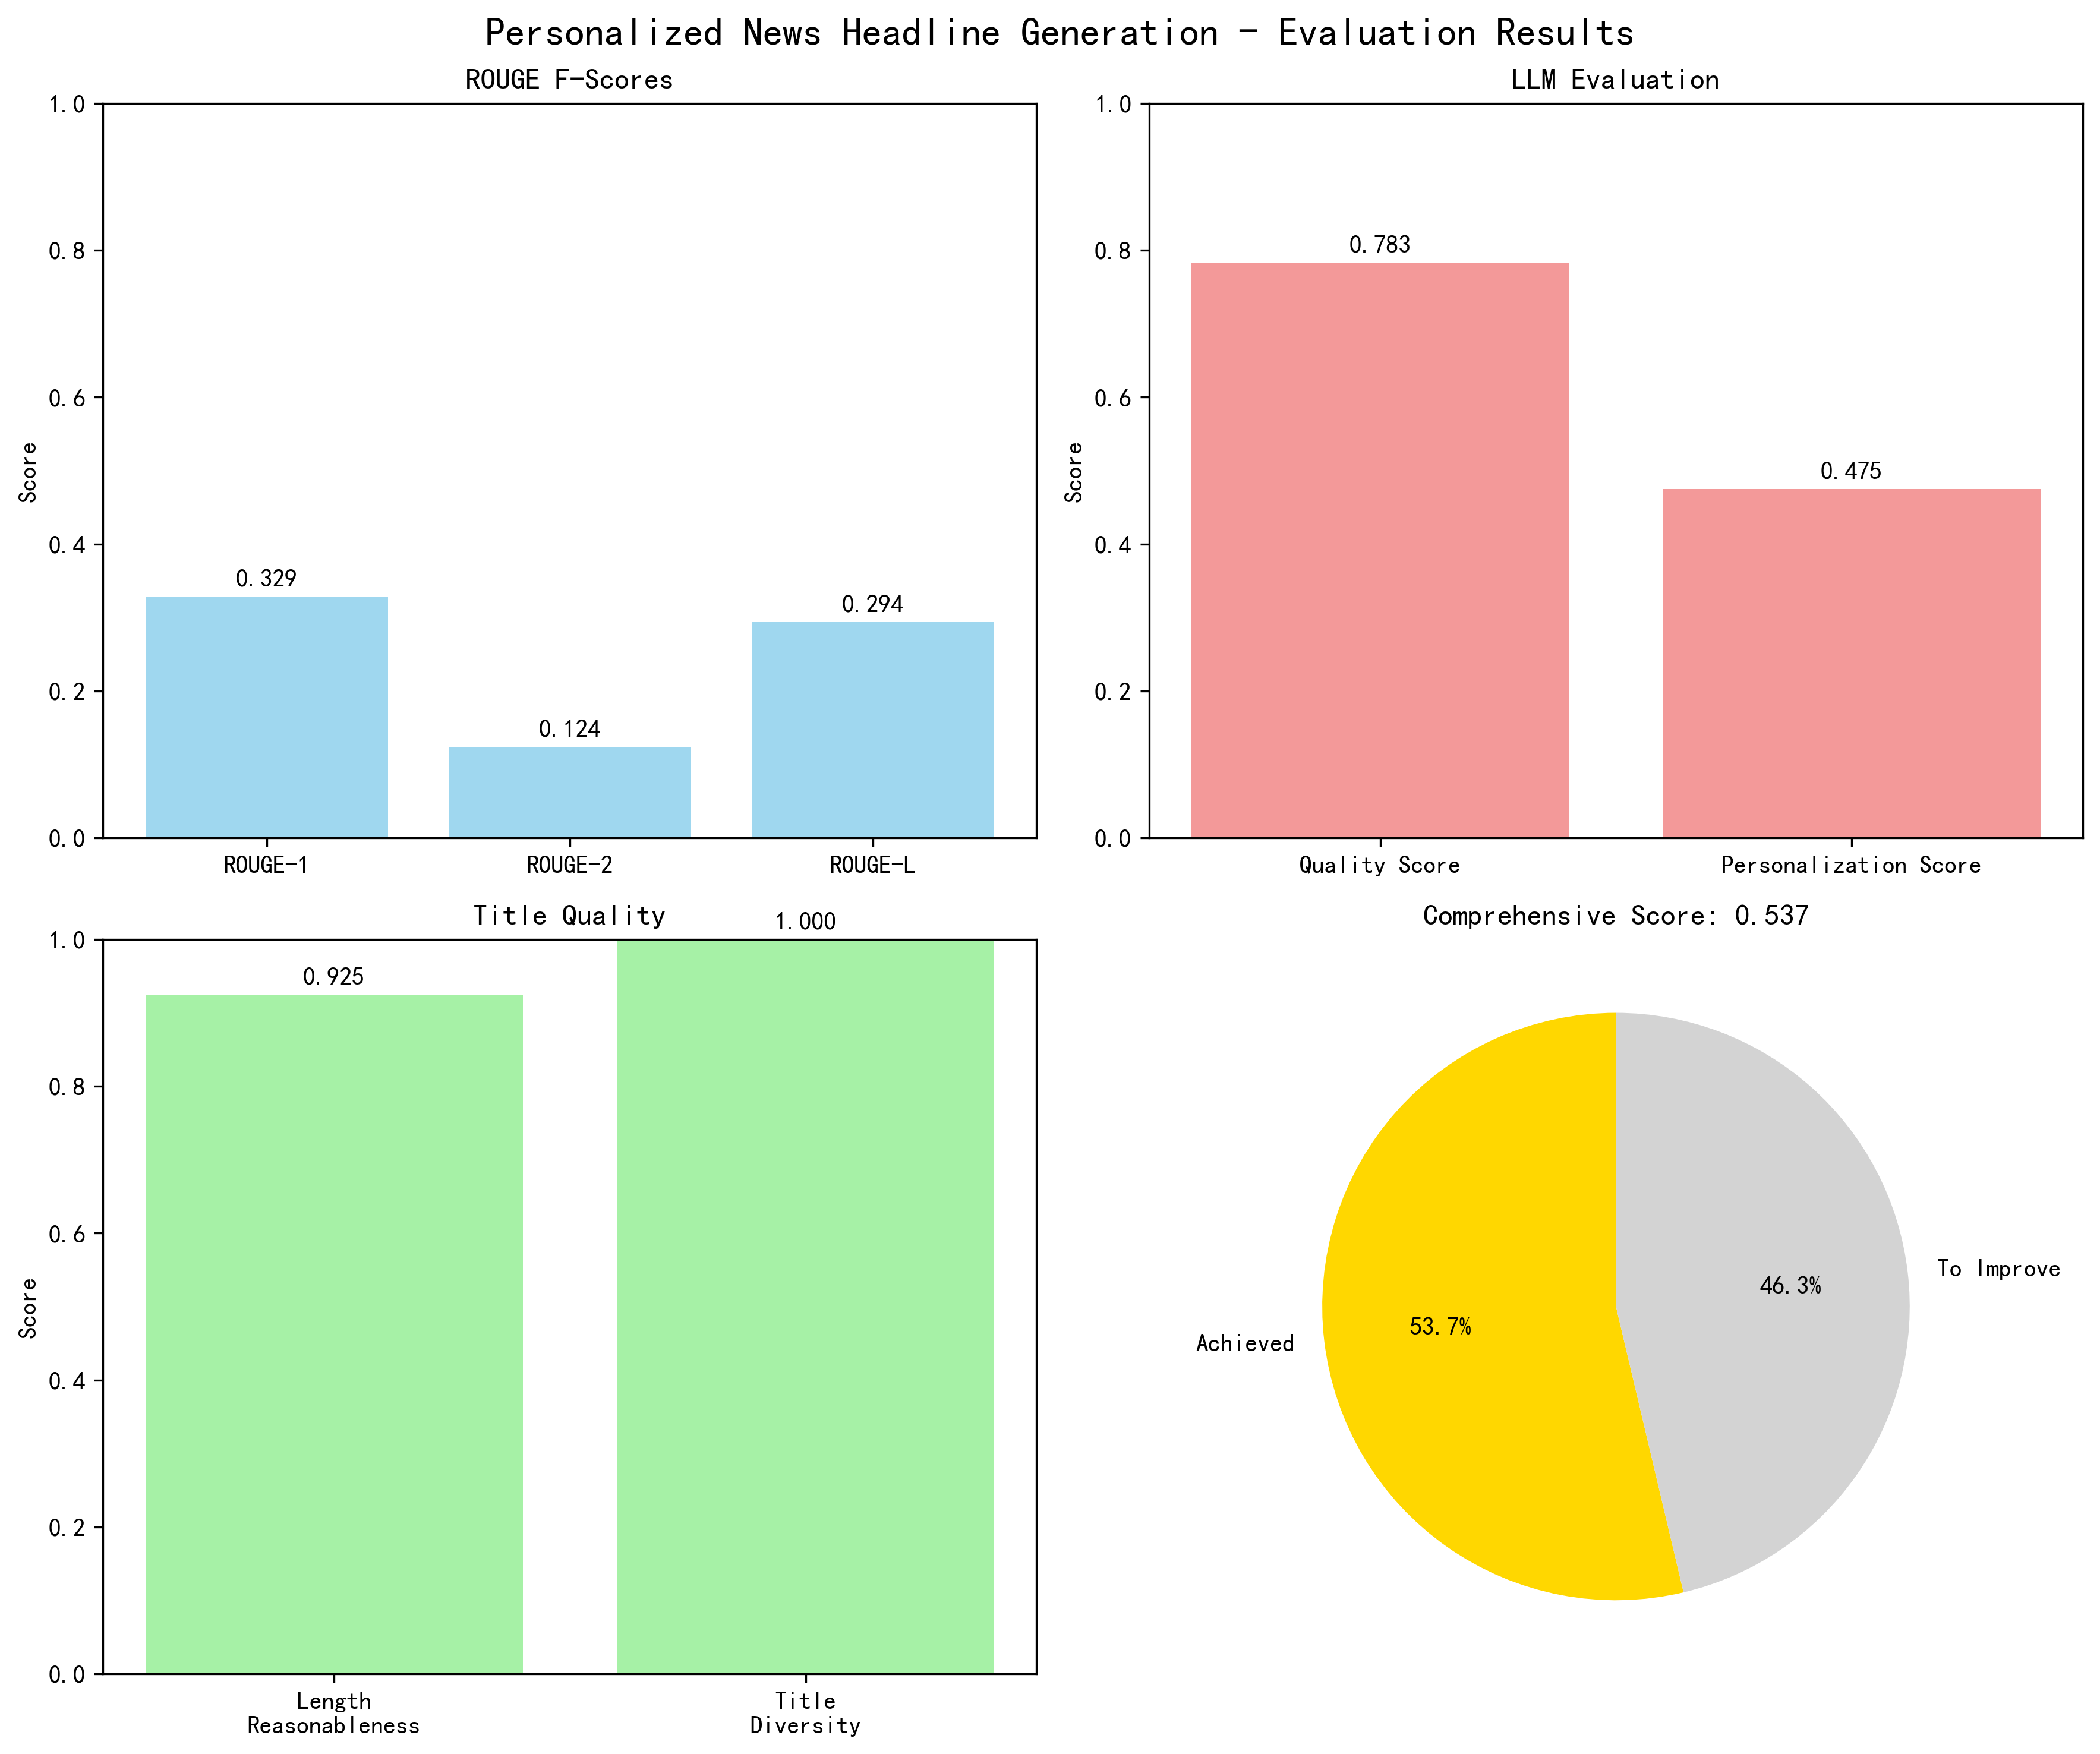
\includegraphics[width=0.68\textwidth]{fig/evaluation_chart_20250622_212308.png}   
  \caption{Prompt Engineering Method Evaluation Results}\label{fig:prompt_evaluation}
\end{figure}

\subsection{Experimental Results}
Based on large language model calls through the ChavAPI platform, this project completed personalized headline generation experiments on test samples. Experiments used DeepSeek-Chat-V3 model as the main generation and evaluation model.

From ROUGE automatic evaluation results, the system achieved ideal performance: \textbf{ROUGE-1 F-score reached 0.3286, ROUGE-2 F-score was 0.1238, and ROUGE-L F-score was 0.2938}. These metrics are significantly higher than the peak performance of the baseline method, indicating that generated personalized headlines have good similarity with reference headlines in terms of vocabulary coverage and language structure.

LLM intelligent evaluation also provided objective and fair assessment of headline generation results. In quality evaluation, the system achieved a comprehensive quality score of 0.783 (out of 1.0), equivalent to 7.83 out of 10, indicating that generated headlines reached high levels in dimensions such as accuracy, attractiveness, and clarity. For personalization evaluation, interest matching reached 0.70, category relevance was 0.5625, and historical consistency was 0.575, demonstrating the system's ability to understand user preferences and generate relevant content.

From specific generation cases, the system can adjust headline expression and emphasis according to users' interest areas. For example, for users focusing on legal and political news, the system generated headline "High-Stakes Legal Battle Erupts Over Trump's Rollback of Obama-Era Pollution Rules" highlighting keywords like "legal battle" and "high-stakes"; for sports enthusiasts, headline "Verlander Scolded by MLB Over Ball-Tampering Claims Ahead of All-Star Game" emphasized specific players and league dynamics. These cases demonstrate the flexibility and precision of prompt engineering in personalized content generation.

In comprehensive scoring, the system achieved a final score of 0.5370 (out of 1.0), with LLM quality evaluation contributing the most (30\% weight, score 0.783), and personalization effect evaluation also performing well (25\% weight, score 0.475). This result validates the effectiveness of the prompt engineering method in balancing content quality and personalization effects.

\section{Comparative Analysis of Two Methods}
Through in-depth analysis and experimental validation of the PENS baseline method and prompt engineering method, comprehensive comparison can be made from multiple dimensions including technical architecture, implementation complexity, performance, and practicality.

\textbf{Technical Architecture Comparison:} The baseline method adopts a traditional deep learning pipeline, including data preprocessing, user encoder training, personalized generator pre-training and fine-tuning, with a relatively complex but logically clear overall architecture. The prompt engineering method adopts a simplified architecture of "data preprocessing + prompt design + LLM calling," avoiding complex model training processes but requiring higher quality prompt design. From a technical advancement perspective, the baseline method embodies classic applications of sequence-to-sequence generation and attention mechanisms, while the prompt engineering method represents emerging technical approaches in the era of large language models.

\textbf{Implementation Complexity Comparison:} The baseline method's environment setup is relatively complex, requiring CUDA environment configuration, GPU memory management, PyTorch version compatibility handling, etc., with high hardware requirements. The training process involves extensive hyperparameter tuning, including learning rate scheduling, batch size optimization, early stopping strategies, etc., requiring strong deep learning background knowledge. The prompt engineering method has a significantly lower implementation threshold, mainly relying on standard Python environments and API calls, without GPU hardware support requirements, with relatively low technical background requirements. However, prompt design itself is an art, requiring deep understanding of the task domain.

\textbf{Performance Comparison:} From ROUGE evaluation metrics, the baseline method can achieve relatively high lexical overlap after training convergence, mainly benefiting from end-to-end training optimization and learning from large amounts of training data. The prompt engineering method's ROUGE scores showed significant improvement (ROUGE-1: 0.3286 vs. baseline method peak 0.2419), also performing more prominently in personalization effects. The baseline method's personalization mainly relies on implicit representations learned by user encoders, while the prompt engineering method can more intuitively integrate user interest information, showing advantages in dimensions like interest matching.

\textbf{Scalability and Generalizability Comparison:} Once the baseline method is trained, model parameters are relatively fixed, and extending to new domains or adapting to new requirements requires retraining, with high costs. The prompt engineering method has stronger flexibility, can quickly adapt to different task requirements by adjusting prompt templates, supporting multi-language and multi-domain extensions. Additionally, as large language model capabilities continue to improve, the prompt engineering method can continuously benefit from foundation model improvements without additional training costs.

\textbf{Resource Consumption and Cost Comparison:} The baseline method's training stage requires substantial computational resources, including GPU training time and power consumption, but the inference stage is relatively efficient. The prompt engineering method shifts computational burden to cloud API services, with low single-call costs, but may face API fee accumulation for large-scale applications. From research and development perspectives, the prompt engineering method enables faster prototype validation and iterative optimization.

\textbf{Interpretability and Controllability Comparison:} The baseline method's neural network structure has certain "black box" characteristics. Although some degree of interpretation is possible through attention weights, the overall decision process is relatively obscure. The prompt engineering method's generation process is more transparent, allowing users to intuitively understand how input information affects output results, facilitating debugging and optimization. In content safety and compliance, the prompt engineering method is also easier to implement precise control.

In summary, both methods have their advantages and are suitable for different application scenarios. The baseline method is more suitable for scenarios with extremely high performance requirements, sufficient data, and abundant computational resources, such as bulk headline generation for large media platforms. The prompt engineering method is more suitable for rapid prototype development, cross-domain applications, and scenarios with high personalization requirements, especially given the continuous improvement of large language model capabilities, its development prospects are broader. From technical development trends, the fusion application of both methods may be an important future direction, utilizing deep learning methods for user representation learning while combining prompt engineering for flexible content generation, balancing performance and system flexibility.

\section{Group Division of Labor}
Shouhe Zhu: Reproduction and improvement of baseline methods, research and analysis of dataset internal structure, writing of report sections 1-2.

Luofan Wang: Design and implementation of prompt engineering methods, construction and optimization of ChavAPI platform, construction of multi-dimensional evaluation system, writing of report sections 3-4.

\end{document}